\begin{Ueberlieferung}% 
{\textit{L}}Konzept: LH XXXVII 3 Bl. 80. 1 Bl. 2\textsuperscript{o}. 2. S. Wasserzeichen.\\%
Cc 2, Nr. 1213 B
\end{Ueberlieferung}
%\vspace*{4mm}% PR: Rein provisorisch !!!
%
% \begin{Datierungsgruende}%
% ?? Wasserzeichen
% \end{Datierungsgruende}
%
\count\Afootins=1200
\count\Bfootins=1000
\count\Cfootins=1200
\vspace{-0.4em}
\pstartfirst%
\noindent%
%\lbrack80~r\textsuperscript{o}\rbrack\ 
[80~r\textsuperscript{o}] 
\edtext{Erit}{\lemma{}\Bfootnote{%
%\lbrack80~r\textsuperscript{o}\rbrack\ \ \textbar \ 
$\displaystyle\frac{CE}{ED}\sqcap\frac{EP}{RQ}\sqcap\frac{ES}{ST}$ \ \textit{gestr.}\ \textbar\ Erit \textit{ L}}}
ergo vis in composita 
\edtext{ratione brachiorum\protect\index{Sachverzeichnis}{brachium} $FE$ $GE$}{\lemma{ratione}\Bfootnote{\textit{(1)}\ potentiarum\protect\index{Sachverzeichnis}{potentia} $AB$ \textit{(2)}\ brachiorum \textit{L}}} 
et rectarum $ER$ $RQ.$ 
\pend
\vspace{1em}% PR: Rein provisorisch !!!
\pstart\noindent
\lbrack \textit{Nachfolgend klein gedruckter Text gestrichen:}\rbrack 
\pend 
\vspace{0.4em}
\pstart
\footnotesize
% \noindent
Comme $CE$ est \`{a} $DE,$ de m\^{e}me doit estre le poids $A,$ au poids $B$ tout le reste estant pos\'{e} le 
\edtext{m\^{e}me.\\\indent Positis $FE,$ et $GE$ aequalibus}{\lemma{m\^{e}me.}\Bfootnote{\textit{(1)}\ Comme \textit{(2)}\ Si circulus describatur, \textit{(a)} cujus radius $A$ \textit{(b)} radio $FE=GE,$ erit  \textit{(3)}\ Positis [...] aequalibus \textit{ L}}}
erunt ut arcus subtensarum, $CE,$ et $ED,$ ita pondera\protect\index{Sachverzeichnis}{pondus} $A$ et $B,$ aut fiat aequilibrium.\protect\index{Sachverzeichnis}{aequilibrium}
\pend
%\vspace{2em}
%\pstart
%\centering
%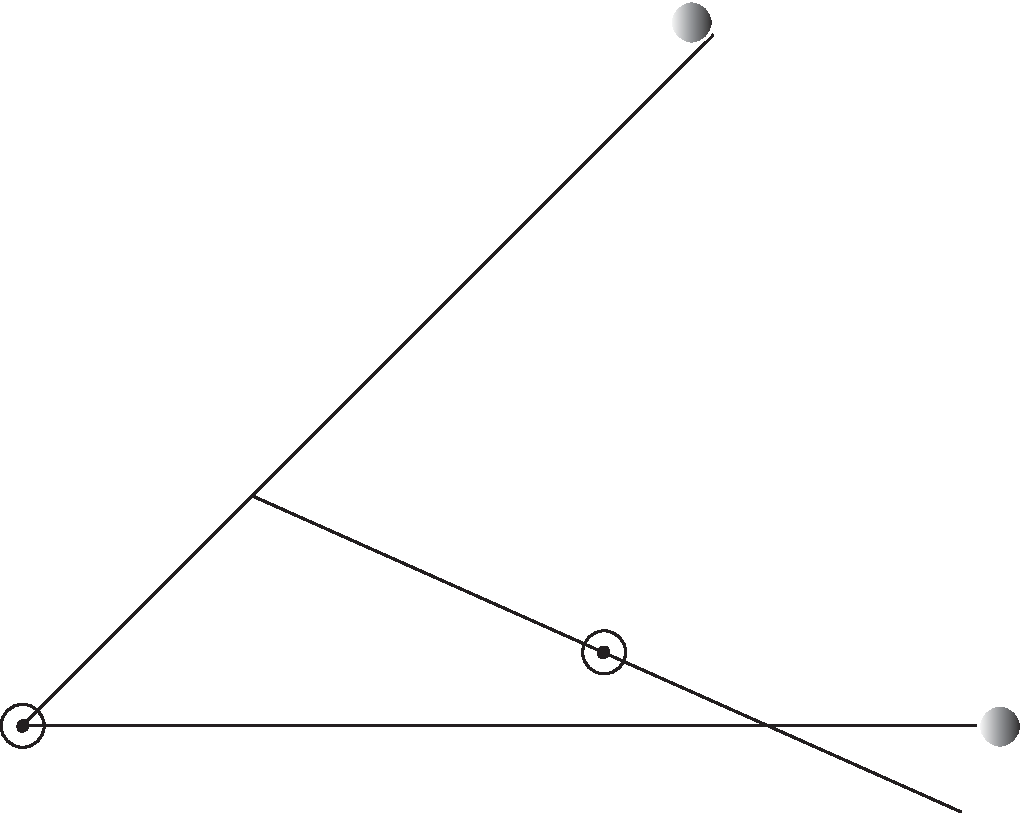
\includegraphics[width=0.36\textwidth]{images/LH037,03_080r-d1.pdf}\\
%\centering[\textit{Fig. 1}]
%\pend
%\newpage
\pstart\footnotesize
\rule[-4mm]{0mm}{0mm}Comme $CE$ est \`{a} $DE,$ de m\^{e}me doit estre le poids $A$ au poids $B$ \`{a} fin qu'il y ait 
\edtext{equilibre. \normalsize Car $\displaystyle\frac{FE}{FH}=\alpha.$ }{\lemma{equilibre.}\Bfootnote{\textit{(1)}\ Les bras\protect\index{Sachverzeichnis}{bras} estant posez \'{e}gaux  \textit{(2)}\ Car \textit{(a)} s'ils sont inegaux \textit{(b)} $\displaystyle\frac{FE}{FH}=\alpha.$ \textit{L}}}\
$\begin{array}{ll} \displaystyle\frac{GE}{GI = FH} = \underset{r}\beta.\left| \begin{array}{c} CEG \ $rectus$ \\ DEF \ $rectus$ \\ GC \ $parallela$ \ FE \end{array}\right| \displaystyle\frac{CE}{ED} = \frac{EL}{LM}. \end{array}$
\edtext{Nam in infinite parvis idem est sive arcum sive ejus loco portionem tangentis sumamus.}{\lemma{}\Bfootnote{Nam [...] sumamus. \textit{ erg.} \textit{L}}} \rule[-4mm]{0mm}{10mm}
\pend
\newpage
\count\Bfootins=1200
\pstart
\centering
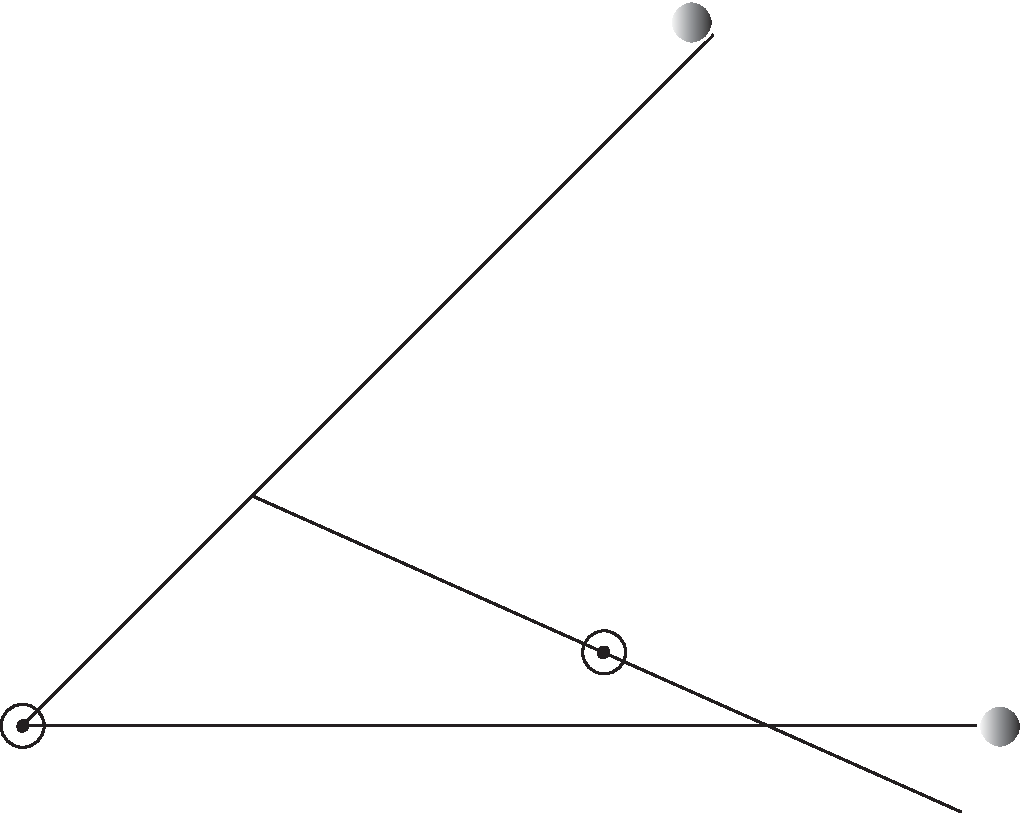
\includegraphics[width=0.34\textwidth]{images/LH037,03_080r-d1.pdf}\\
\centering[\textit{Fig. 1}]
\pend
\vspace{1.5em}
\pstart
$\displaystyle HN \setline{1}= \frac{LM}{\alpha} \quad IP =  \displaystyle\frac{EL}{\beta} \quad  \displaystyle\frac{IP}{HN} = \begin{array}{cc}  \displaystyle\frac{EL}{\beta} \\ \hline\hline  \displaystyle\frac{LM}{\alpha} \end{array} =  \displaystyle\frac{EL \smallfrown  \alpha}{LM \smallfrown  \beta}.$
\pend
\pstart%
Ergo $\displaystyle\frac{CE}{ED}{\smallfrown \atop}\frac{a}{b}=\frac{IP}{HN}.$
Jam \rule[-4mm]{0mm}{10mm}$\displaystyle\frac{\alpha}{\beta}=\frac{FE}{GE}$.
\pend
%\vspace{1.5em}
%\pstart
%\centering
%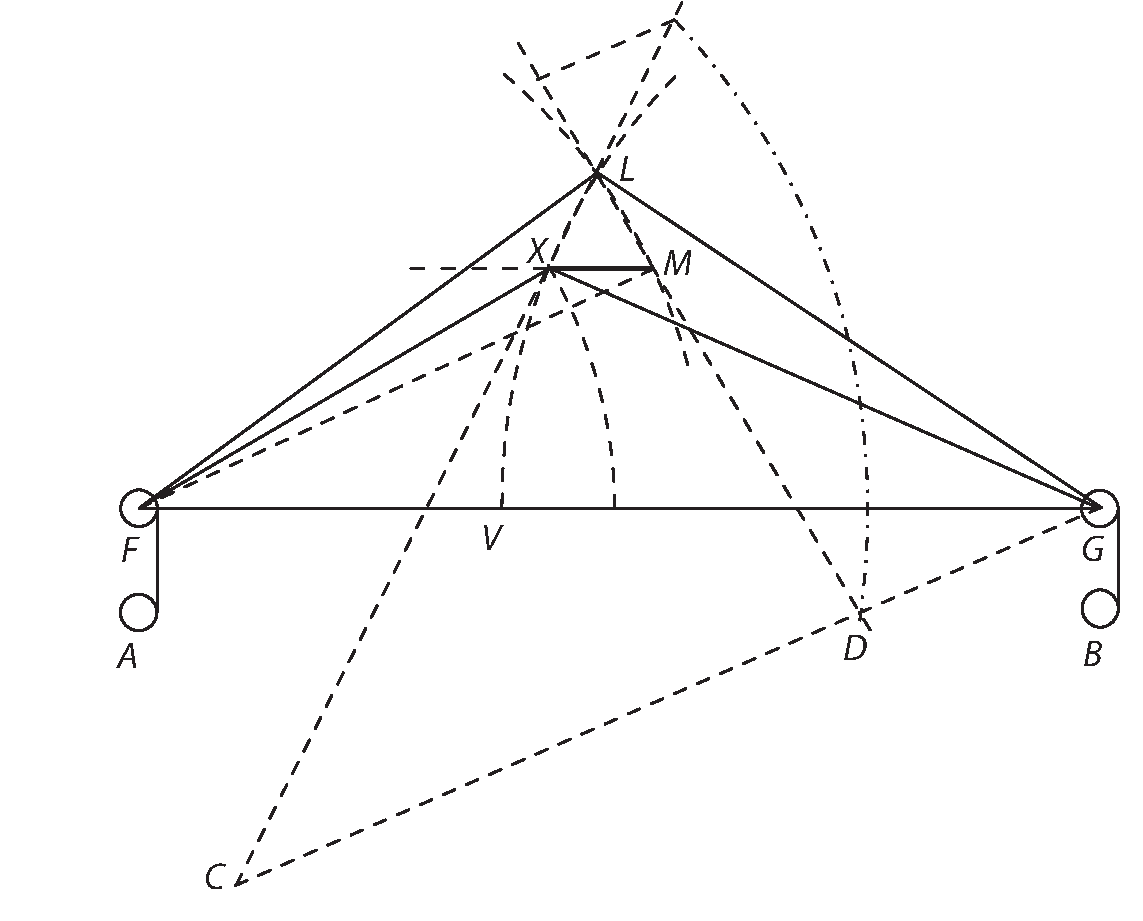
\includegraphics[width=0.76\textwidth]{images/LH037,03_080r-d2.pdf}\\
%\centering [\textit{Fig. 2}]
%\pend
%\vspace*{2mm}
\pstart
Ergo\rule[-4mm]{0mm}{10mm} $\displaystyle\frac{CE}{ED}{\smallfrown \atop}\frac{FE}{GE}=\edtext{\frac{IP}{HN}$.
\edtext{}{\lemma{}\Afootnote{\textit{Unterhalb des gestrichenen Texts}: invertendum\vspace{-4mm}}}%
Nam vires ut anguli, anguli vero in directa ratione arcuum, et reciproca radiorum arcus autem sunt ut $ED$ $EC$ quare $\displaystyle A\sqcap\frac{GE, ED}{FE, CE}$.
\protect\rule[-4mm]{0mm}{10mm}$\displaystyle\frac{A}{B}=\frac{CE\smallfrown FE}{ED\smallfrown GE}$ erit aequilibrium\protect\index{Sachverzeichnis}{aequilibrium}%
}{\lemma{$\displaystyle\frac{IP}{HN}$.}\Bfootnote{\textit{(1)}\ Ergo debent pondera\protect\index{Sachverzeichnis}{pondus}\ \textit{(a)} $\beta$\ \textit{(b)} esse\ \textit{(2)}\ Quare si $\displaystyle\frac{A}{B}=\frac{HN}{\cancel{IP}}$ habebitur aequlibrium\ \textit{(3)}\  Nam [...] aequilibrium \textit{ L}}}
\edtext{vel potentiae\protect\index{Sachverzeichnis}{potentia} $A$ exercitium ad exercitium potentiae $B$ erit ut $FE, CE$ ad $ED, GE$.}{\lemma{}\Bfootnote{vel [...] $GE$ \textit{erg.} \textit{L}}} 
\pend
\pstart
Loco \rule[-4mm]{0mm}{10mm}$\displaystyle\frac{CE}{ED}$ substitui potest $\displaystyle\frac{EG}{GD}$ pro $\bigtriangledown$li $DGE$, et $DEC$ similia item $\displaystyle\frac{CE}{ED}\sqcap\frac{ER}{RQ}\sqcap\frac{ES}{ST}$.
\pend
\pstart
Si $FE$ $EG$ coincidant in unam rectam $FG,$ 
\edtext{erit potentia}{\lemma{erit}\Bfootnote{\textit{(1)}\ vis ad \textit{(2)}\ potentia \textit{L}}} seu gravitatio\protect\index{Sachverzeichnis}{gravitatio} ipsius $A$ ad potentiam seu gravitationem ipsius 
\edtext{$B$, reciproce}{\lemma{$B$,}\Bfootnote{\textit{(1)}\ ut idem ad seipsum quod est absurdum. Unde error in ratiocinatione latere debet. Is in eo consistit  \textit{(2)}\ reciproce \textit{L}}} 
ut $FE$ ad $EG$ tunc enim fit $CE\sqcap ED$ cum angulus \textit{FEG} infinite obtusus. Idque verum esse aliunde 
constat.%
\edlabel{LH037,03_080r_xy-1}%
\edtext{}{{\xxref{LH037,03_080r_xy-1}{LH037,03_080r_xy-2}}\lemma{constat.}\Bfootnote{%
\textit{(1)}~Superest ut videamus quomodo dens sive vectis ducendus figuram debeat, ut semper eadem vi duceatur %
\textit{(2)}~Quid [...] curva, \textit{L}}}
\pend
\pstart
\centering
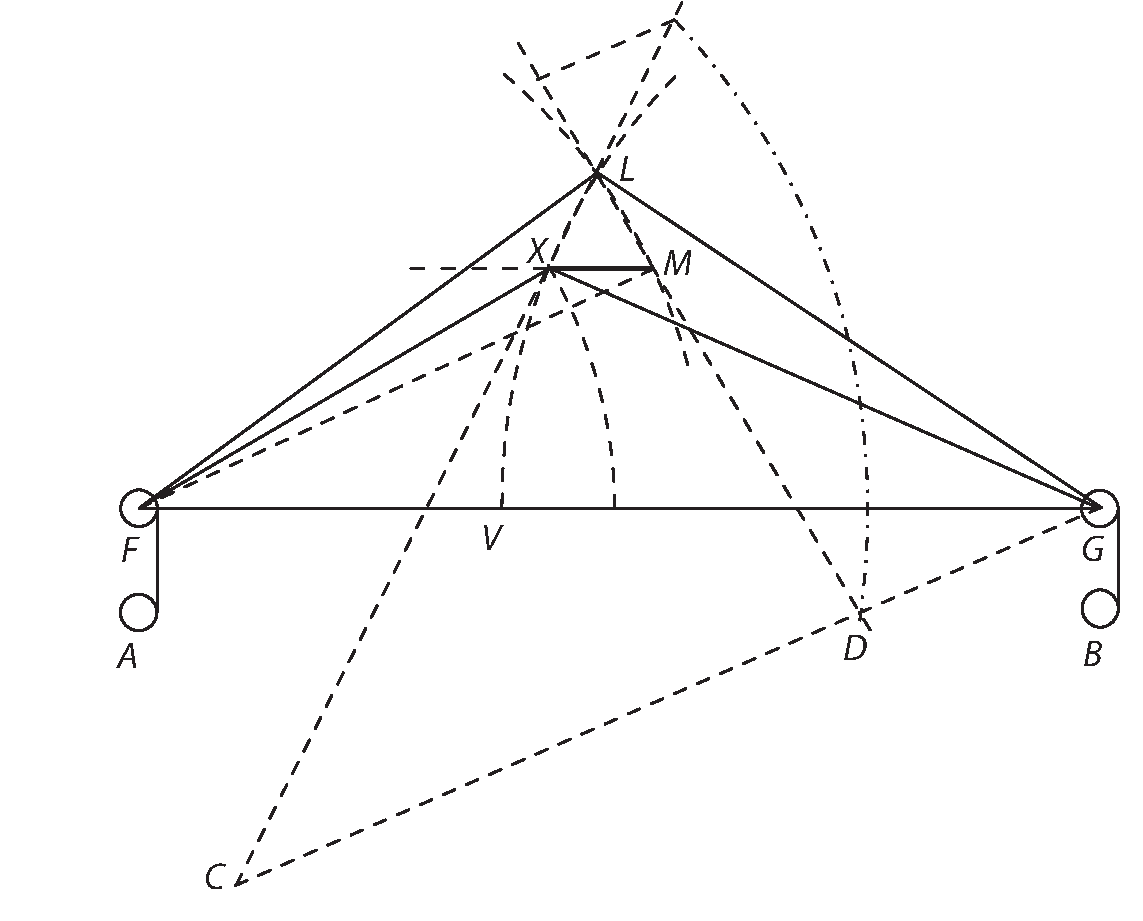
\includegraphics[width=0.76\textwidth]{images/LH037,03_080r-d2.pdf}\\
\centering [\textit{Fig. 2}]
\pend
\vspace{2em}
\pstart
Quid \setline{1} si dens seu vectis\protect\index{Sachverzeichnis}{vectis} dicendus sit linea curva,%
\edlabel{LH037,03_080r_xy-2}
ut \textit{FXM.} 
Tum patet eodem modo ducendas perpendiculares tum ex $FM$ nempe $LD$
\edtext{(vel $MD$)}{\lemma{(vel $MD$)}\Bfootnote{\textit{erg.} \textit{L}}}
tum
\edtext{\lbrack\edtext{}{\lemma{\lbrack$GM$}\Cfootnote{Eckige Klammer von Leibniz.}}%
$GM$ vel $GX$ (nam differentia infinite
\edtext{parva\phantom(\hspace{-1.2mm})\rbrack.}{\lemma{parva\phantom(\hspace{-1.2mm})\rbrack}\Cfootnote{Eckige Klammer von Leibniz.}}%
}{\lemma{$\lbrack GM$}\Bfootnote{\textit{(1)}\ nempe \textit{(2)}\ (\phantom)\hspace{-1.2mm}nam differentia in $GX$ \textit{(3)}\ vel $GX$ [...] parva\phantom(\hspace{-1.2mm})\rbrack. \textit{L}}} 
nempe $L$ $C,$ donec occurrant rectae $GDC$ quae sit parallela ipsi $XM$ tangenti curvae et fore
potentiam $A$ ad potentiam $B$ in composita ratione ex $FM$ ad $GM$ et $MD$ (sive $LD$) ad $MC$ (sive 
\edtext{$LC$).\\\indent Id est ex}{\lemma{$LC$).}\Bfootnote{ \textit{(1)}\ Hinc \textit{(2)}\ Id est ex  \textit{ L}}} puncto in curva dato $M$ ducantur rectae $MF$ $MG$ et ad has perpendiculares $MD$ $MC$ parallelae tangentis occurrentes erit ratio potentiarum composita ex $MF$ ad $MG,$ et $MD$ ad $MC$ quae ratio si semper aequalis cuidam datae, erit curva talis, ut semper aequalis sit actio, quaeritur qualis ea curva.
\pend
\count\Afootins=1500
\count\Bfootins=1500
\count\Cfootins=1500
\pstart
\centering
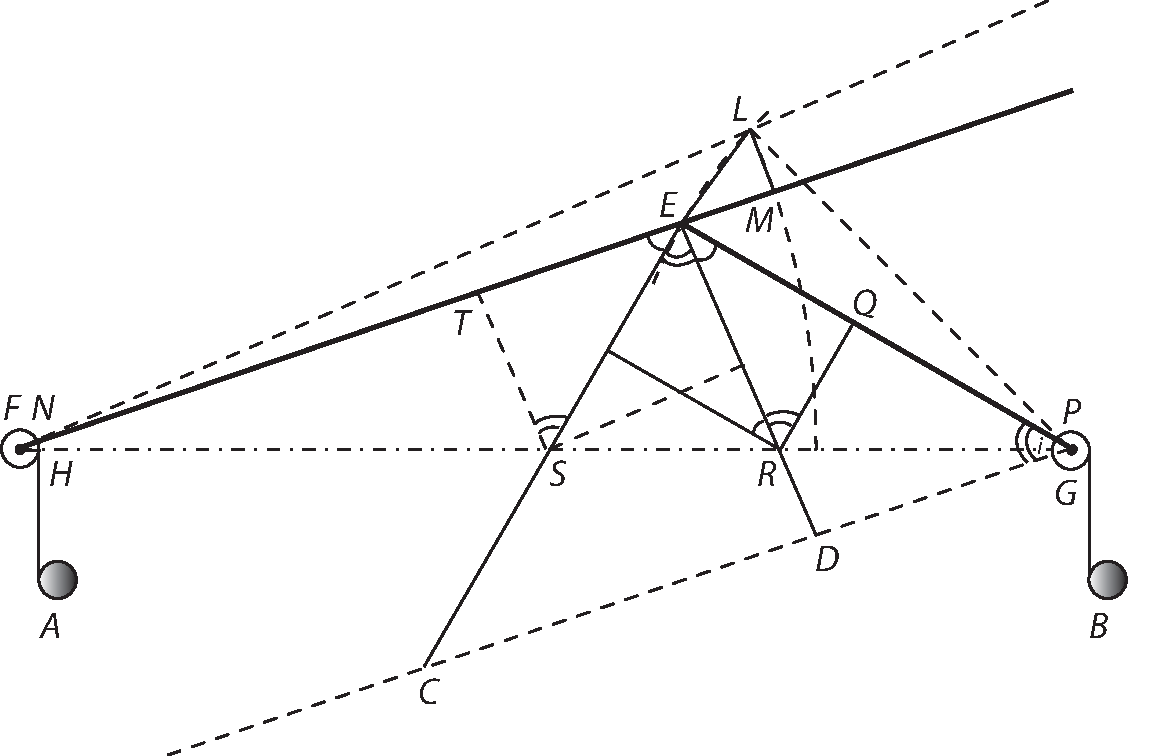
\includegraphics[width=0.88\textwidth]{images/LH037,03_080r-d3.pdf}\\
\centering [\textit{Fig. 3}]
\pend
\vspace{1.5em}